\documentclass[11pt]{article}

\usepackage[a4paper,margin=25mm]{geometry}
\usepackage[T1]{fontenc}
\usepackage[utf8]{inputenc}
\usepackage{lmodern}
\usepackage{microtype}
\usepackage{amsmath,amssymb,amsthm,mathtools}
\usepackage{bm}
\usepackage{booktabs}
\usepackage{threeparttable}
\usepackage{tabularx}
\newcolumntype{Y}{>{\raggedright\arraybackslash}X}
\newcolumntype{P}[1]{>{\raggedright\arraybackslash}p{#1}}
\usepackage{graphicx}
\usepackage{float}
\usepackage{placeins}
\usepackage{enumitem}
\usepackage[round,authoryear]{natbib}
\usepackage{xcolor}
\usepackage{url}
\usepackage{setspace}
\usepackage{caption}
\usepackage{subcaption}
\usepackage{fancyhdr}
\usepackage{hyperref}
\makeatletter
\DeclareRobustCommand{\MainRef}[2]{\hyper@linkfile{#2}{main.pdf}{#1}}
\makeatother
\setlength{\headheight}{14pt}

\definecolor{linkblue}{RGB}{32,83,130}
\hypersetup{
  colorlinks=true,
  linkcolor=linkblue,
  citecolor=linkblue,
  urlcolor=linkblue,
  filecolor=linkblue,
  pdftitle={Appendix to Blockwise Occupancy Inference under Weak Dependence with Record-Based Persistence Thresholds},
  pdfauthor={Charbel Al Tannoury, Anis Hoayek, Youssef Salman, Hyam Abboud, Mireille Batton-Hubert},
  pdfkeywords={change-point detection, record indicators, local asymptotic normality, absolute regularity, Poisson-binomial approximation, CHARN models}
}

\setstretch{1.00}
\setlength{\parskip}{3pt}
\setlength{\parindent}{15pt}
\setlist{nosep,leftmargin=*}
\captionsetup{font=small,labelfont=bf}
\renewcommand{\topfraction}{0.9}
\renewcommand{\textfraction}{0.08}
\renewcommand{\floatpagefraction}{0.8}
\setcounter{topnumber}{3}
\brokenpenalty=10000

\newtheorem{theorem}{Theorem}[section]
\newtheorem{proposition}[theorem]{Proposition}
\newtheorem{corollary}[theorem]{Corollary}
\newtheorem{lemma}[theorem]{Lemma}
\theoremstyle{definition}
\newtheorem{definition}[theorem]{Definition}
\newtheorem{assumption}[theorem]{Assumption}
\newtheorem{example}[theorem]{Example}
\theoremstyle{remark}
\newtheorem{remark}[theorem]{Remark}

\DeclareMathOperator{\PB}{PB}
\DeclareMathOperator{\Bin}{Bin}
\DeclareMathOperator{\Var}{\mathbb{V}}
\DeclareMathOperator{\Cov}{Cov}
\DeclareMathOperator{\diag}{diag}
\DeclareMathOperator{\argmax}{arg\,max}
\DeclareMathOperator{\argmin}{arg\,min}
\DeclareMathOperator{\TV}{TV}
\newcommand{\Prob}{\mathbb P}
\newcommand{\E}{\mathbb E}
\newcommand{\R}{\mathbb R}
\newcommand{\1}{\mathbf 1}
\newcommand{\cF}{\mathcal F}
\newcommand{\cL}{\mathcal L}
\newcommand{\cM}{\mathcal M}
\newcommand{\cP}{\mathcal P}
\newcommand{\eps}{\varepsilon}
\newcommand{\dd}{\,\mathrm d}
\newcommand{\KL}{D_{\mathrm{KL}}}

\pagestyle{fancy}
\fancyhf{}
\fancyhead[L]{\small Blockwise occupancy under weak dependence}
\fancyhead[R]{\small Al Tannoury et al.}
\fancyfoot[C]{\thepage}
\renewcommand{\headrulewidth}{0.3pt}

\title{\bfseries Appendix to\\[3pt] Blockwise Occupancy Inference under Weak Dependence with Record-Based Persistence Thresholds}

\author{
Charbel Al Tannoury$^{1,*}$, Anis Hoayek$^{1}$, Youssef Salman$^{1}$,\\
Hyam Abboud$^{2}$, and Mireille Batton-Hubert$^{1}$\\[5pt]
\small $^{1}$Mathematical and Industrial Engineering Department, Mines Saint-Etienne,\\[-2pt]
\small CNRS, UMR 6158 LIMOS, Institut Henri Fayol, F-42023 Saint-Etienne, France\\
\small $^{2}$Department of Mathematics, Lebanese University, Fanar-Matn, P.O. Box 90656, Lebanon\\[3pt]
\small $^*$Corresponding author: \href{mailto:charbel.altannoury@emse.fr}{charbel.altannoury@emse.fr}
}

\date{}

\begin{document}
\renewcommand{\thesection}{\Alph{section}}
\renewcommand{\theequation}{A\arabic{equation}}
\renewcommand{\thetable}{A\arabic{table}}
\renewcommand{\thefigure}{A\arabic{figure}}
\renewcommand{\thepage}{A\arabic{page}}
\maketitle
\noindent This appendix contains the coupling and CHARN proofs, extended simulation analyses, and the full CWRU application results. References to unprefixed sections, equations, and results refer to the main manuscript.
\section{Vector coupling lemma and classification proof}\label{app:coupling}

\begin{lemma}[Vector Berbee coupling]\label{lem:vectorberbee}
Let $Y_1,\ldots,Y_m$ be random elements of standard Borel spaces. On an extension of the probability space there exist mutually independent $Y_1^*,\ldots,Y_m^*$, with $\cL(Y_j^*)=\cL(Y_j)$ for every $j$, such that
\[
\Prob\{(Y_1,\ldots,Y_m)\ne(Y_1^*,\ldots,Y_m^*)\}
\le\sum_{j=2}^m
\beta\{\sigma(Y_1,\ldots,Y_{j-1}),\sigma(Y_j)\}.
\]
\end{lemma}

\begin{proof}
We compare the joint vector law with the product of its marginals. Write $\mu_j=\cL(Y_1,\ldots,Y_j)$, $\nu_j=\cL(Y_j)$, and $\pi_j=\bigotimes_{i=1}^j\nu_i$. With the total-variation convention used in this paper,
\[
d_{\TV}(\mu_j,\mu_{j-1}\otimes\nu_j)
=\beta\{\sigma(Y_1,\ldots,Y_{j-1}),\sigma(Y_j)\}.
\]
Tensoring both measures with the same probability law does not change total variation. We can therefore use the triangle inequality to obtain the recursion
\[
d_{\TV}(\mu_j,\pi_j)
\le d_{\TV}(\mu_{j-1},\pi_{j-1})
+\beta\{\sigma(Y_1,\ldots,Y_{j-1}),\sigma(Y_j)\}.
\]
Iterating this inequality, we bound $d_{\TV}(\mu_m,\pi_m)$ by the displayed sum.

It remains to realize this comparison as a coupling. A maximal coupling of the two vector laws $\mu_m$ and $\pi_m$ exists on standard Borel spaces and has mismatch probability $d_{\TV}(\mu_m,\pi_m)$. The second vector has product law $\pi_m$, so its coordinates are mutually independent and have the required marginals. This is the vector form of Berbee's coupling lemma \citep{berbee1979random}.
\end{proof}

\begin{proof}[Proof of Theorem~\MainRef{theorem.3.8}{3.8}]\hypertarget{proof:thm:classification}{}
We work first with the independent Bernoulli surrogate $S^*=\sum_{j=1}^mY_j^*$ from Theorem~\MainRef{theorem.3.2}{3.2}. For $\lambda>0$,
\[
\E e^{\lambda S^*}=\prod_{j=1}^m\{1-p_{b,j}+p_{b,j}e^\lambda\}.
\]
To replace the individual success probabilities by their average, we use the concavity of the logarithm of each factor as a function of $p_{b,j}$. Jensen's inequality gives
\[
\E e^{\lambda S^*}
\le\{1-\bar p_b+\bar p_be^\lambda\}^m.
\]
Optimizing the resulting Chernoff bound gives
\[
\Prob(S^*\ge mx)\le e^{-m\KL(x\Vert\bar p_b)}
\quad(x>\bar p_b),
\qquad
\Prob(S^*\le mx)\le e^{-m\KL(x\Vert\bar p_b)}
\quad(x<\bar p_b),
\]
at the integer values used below.

We now identify the error event for each label. For the reference label, the error event is $\{S^*\ge a_m+1\}=\{S^*\ge m u_m\}$. For the elevated label, it is the union of $\{S^*\le a_m\}=\{S^*\le m\ell_m\}$ and $\{S^*\ge k_m\}=\{S^*\ge m v_m\}$. For the high-occupancy label, it is $\{S^*\le k_m-1\}=\{S^*\le m w_m\}$. Applying the corresponding tail bounds gives the three expressions, with a union bound for the two elevated-label errors. The lower-tail bound is obtained by repeating the exponential argument with $\lambda<0$. Finally, we return to the dependent count. Theorem~\MainRef{theorem.3.2}{3.2} changes the probability of each complete error event by at most one $\eps_{\mathrm{mix},b}$, which proves (\MainRef{equation.31}{31})-(\MainRef{equation.33}{33}).
\end{proof}

\section{CHARN drift, minorization, and initialization}\label{app:charnmixing}

\begin{proof}[Proof of Proposition~\MainRef{theorem.7.4}{7.4}]\hypertarget{proof:prop:orderpdrift}{}
We first construct a quadratic drift function adapted to the lag shifts. Write \(u(z)=(z_1^2,\ldots,z_p^2)^\top\) and choose
\(\rho(B_c)<\lambda_0<1\). The positive vector defined by the convergent Neumann series
\begin{equation}\label{eq:charnweights}
w=(I-B_c^\top/\lambda_0)^{-1}\mathbf1_p
=\sum_{k\ge0}(B_c^\top/\lambda_0)^k\mathbf1_p
\end{equation}
satisfies \(w\ge\mathbf1_p\) and \(B_c^\top w=\lambda_0(w-\mathbf1_p)\le\lambda_0w\).
Using the centered unit-variance innovations and equation~(\MainRef{equation.59}{59}), we obtain
\[
\E\{u(Z_t)\mid Z_{t-1}=z\}\le A\mathbf e_1+B_cu(z).
\]
Hence \(W(z)=1+w^\top u(z)\) obeys
\[
P_\vartheta W(z)\le1+Aw_1+\lambda_0w^\top u(z)
=\lambda_0W(z)+(1+Aw_1-\lambda_0)
\]
uniformly in the parameter.

We next verify the small-set condition. Fix a sublevel set \(C_R\) and a target rectangle \(K_L=[-L,L]^p\).
Write \(y_1,\ldots,y_p\) for the next \(p\) generated observations and
\(z^{(k)}=(y_k,z_1^{(k-1)},\ldots,z_{p-1}^{(k-1)})\).
The triangular change of variables from innovations to observations has
Jacobian \(\prod_{k=1}^p V_\eta(z^{(k-1)})\).
The transition density, with terminal coordinates reversed, is consequently
\begin{equation}\label{eq:triangular-density}
\prod_{k=1}^p
\frac1{V_\eta(z^{(k-1)})}
f\!\left(\frac{y_k-T_\theta(z^{(k-1)})}{V_\eta(z^{(k-1)})}\right).
\end{equation}
When \(z\in C_R\), the terminal state belongs to \(K_L\), and the parameter ranges over its compact set, every intermediate state belongs to a common compact set. Joint continuity and the positive lower scale bound give
\[
0<\underline v\le V_\eta(z^{(k)})\le\overline v<\infty,
\qquad |T_\theta(z^{(k)})|\le\overline T.
\]
The innovation arguments therefore remain in a compact interval. The minimum of \(f\) on it is positive, so equation~\eqref{eq:triangular-density} has a uniform positive lower bound on \(C_R\times K_L\). Taking normalized Lebesgue measure on \(K_L\), we obtain the \(p\)-step minorization, with a measure independent of the parameter.

For \(p+1\) transitions, we integrate the first generated observation over a fixed compact interval of positive length. The same compactness argument applies to all \(p+1\) factors and supplies a positive lower bound on the same terminal rectangle. This gives the consecutive minorization on a common target set. Finally, positivity of the \(p\)-step density on all of \(\mathbb R^p\) proves Lebesgue irreducibility. In particular, choosing the target rectangle to contain a nonempty sublevel set also gives the required aperiodicity.
\end{proof}

\begin{proof}[Proof of Proposition~\MainRef{theorem.7.5}{7.5}]\hypertarget{proof:prop:explicitdrift}{}
We choose \(\zeta>0\) sufficiently small that
\(\lambda_0=(1+\zeta)c_T^2+c_V<1\). The growth bounds then give
\[
\E(X_t^2\mid X_{t-1}=x)
=T_\theta(x)^2+V_\eta(x)^2
\le(1+\zeta^{-1})A_T^2+A_V+\lambda_0x^2.
\]
Thus \(W(x)=1+x^2\) satisfies the stated drift inequality. For the one- and two-step compact minorizations, we specialize the compact-density argument in the preceding proof to \(p=1\).
\end{proof}

\begin{proof}[Proof of Proposition~\MainRef{theorem.7.6}{7.6}]\hypertarget{proof:prop:charnmixing}{}
The common drift and small-set bounds allow us to apply the drift-minorization theorem \citep[Chapters 15--16]{meyn2009markov}. We obtain uniform geometric ergodicity, with a unique invariant law \(\pi_\vartheta\) satisfying
\begin{equation}\label{eq:Vuniform}
\|P_\vartheta^h(z,\cdot)-\pi_\vartheta\|_{\rm TV}
\le M W(z)\bar\rho^h,\qquad
\pi_\vartheta(W)\le b/(1-\lambda),
\end{equation}
with constants uniform over the parameter family. If the rate is initially obtained for a \(p\)-step skeleton, we write \(h=pn+s\), \(0\le s<p\), and use contraction under \(P_\vartheta^s\). Then
\(\rho_p^n\le\rho_p^{-1}(\rho_p^{1/p})^h\), which gives the claimed raw-time rate after increasing \(M\).

We now pass from transition probabilities to absolute regularity. For a stationary Markov chain on a standard Borel state space, the conditional-law representation and the Markov property give
\begin{equation}\label{eq:markovbeta}
\beta_Z(h)\le
\int\|P_\vartheta^h(z,\cdot)-\pi_\vartheta\|_{\rm TV}\,
\pi_\vartheta(\dd z).
\end{equation}
Indeed, the future path is obtained from its initial state by a common probability kernel, and total variation contracts under that kernel. The bound therefore controls the full past and future sigma-fields, as required. We integrate equation~\eqref{eq:Vuniform} to obtain \(C=M b/(1-\lambda)\). Since \(X_t\) is a coordinate of \(Z_t\), \(\beta_X(h)\le\beta_Z(h)\). Proposition~\MainRef{theorem.3.1}{3.1} and Theorem~\MainRef{theorem.3.2}{3.2} then give the diagnostic count bound with raw support \(r_{\rm eff}\).
\end{proof}

\begin{proof}[Proof of Proposition~\MainRef{theorem.7.8}{7.8}]\hypertarget{proof:prop:charnburnin}{}
At time \(\tau+s\), the state law is \(\mu P_\vartheta^s\). We use the same conditional-law representation as in the stationary case, inserting \(\pi_\vartheta\) in the triangle inequality. This gives
\[
\begin{split}
\beta_{\mu,\vartheta}(s,h)
&\le\int\|P_\vartheta^h(z,\cdot)-\mu P_\vartheta^{s+h}\|_{\rm TV}
\,\mu P_\vartheta^s(\dd z)\\
&\le M\bar\rho^h\,\mu P_\vartheta^s(W)
+M\mu(W)\bar\rho^{s+h}.
\end{split}
\]
The drift inequality implies
\(\mu P_\vartheta^s(W)\le\mu(W)+b/(1-\lambda)\).
Therefore \(C_\mu=M\{2\mu(W)+b/(1-\lambda)\}\) is a uniform finite constant in equation~(\MainRef{equation.65}{65}).

We turn next to the marginal exceedance probabilities. Let \(K_{r_{\rm eff}}\) map the state immediately before a diagnostic's raw support to its exceedance indicator. For \(d=t-r_{\rm eff}-\tau\ge0\), contraction under this kernel gives
\[
|\Prob_\mu(e_t=1)-p_\vartheta|
\le\|\mu P_\vartheta^d-\pi_\vartheta\|_{\rm TV}
\le M\mu(W)\bar\rho^d.
\]
This is the required marginal bound.

To compare the count with its stationary binomial law, we first use vector coupling. It gives the Poisson-binomial approximation with allowance
\((m-1)C_\mu\bar\rho^{q-r_{\rm eff}+1}\).
We then change the marginal parameters of the independent Bernoulli variables to \(p_\vartheta\) at cost at most
\[
\sum_{j=1}^m|\Prob_\mu(e_{t_{b,j}}=1)-p_\vartheta|
\le M\mu(W)\bar\rho^{d_b}
\frac{1-\bar\rho^{mq}}{1-\bar\rho^q}.
\]
Combining these two comparisons by the triangle inequality proves equation~(\MainRef{equation.67}{67}).
\end{proof}

\section{Additional fitted-model comparisons}\label{app:additional}
Table~\ref{tab:additional} gives the remaining competitors from the same fitted-reference experiment. The complete CSV includes replication-level Monte Carlo standard errors for each reported probability.
\begin{table}[htbp]
\centering\small
\caption{Additional comparators under the same reference-block calibration. The definitions and error budgets are those of Section~\MainRef{section.8}{8}.}\label{tab:additional}
\resizebox{\textwidth}{!}{\begin{tabular}{lrrrrr}
\toprule
Scenario / method & $0\to +$ & $0\to2$ & $1\to1$ & $1\to2$ & $2\to2$ \\
\midrule
Gaussian mean 0.40 / Capped energy & 0.050 & 0.009 & 0.363 & 0.363 & 0.921 \\
Gaussian mean 0.40 / Interval scan & 0.048 & 0.010 & 0.000 & 1.000 & 0.996 \\
Gaussian mean 0.40 / Run statistic & 0.050 & 0.010 & 0.022 & 0.963 & 0.426 \\
Gaussian mean 0.55 / Capped energy & 0.050 & 0.010 & 0.359 & 0.360 & 1.000 \\
Gaussian mean 0.55 / Interval scan & 0.051 & 0.011 & 0.000 & 1.000 & 1.000 \\
Gaussian mean 0.55 / Run statistic & 0.053 & 0.010 & 0.033 & 0.953 & 0.832 \\
Student mean 0.40 / Capped energy & 0.051 & 0.011 & 0.353 & 0.348 & 0.974 \\
Student mean 0.40 / Interval scan & 0.051 & 0.012 & 0.002 & 0.996 & 0.999 \\
Student mean 0.40 / Run statistic & 0.050 & 0.009 & 0.057 & 0.917 & 0.552 \\
Student mean 0.55 / Capped energy & 0.051 & 0.010 & 0.359 & 0.332 & 1.000 \\
Student mean 0.55 / Interval scan & 0.051 & 0.009 & 0.004 & 0.995 & 1.000 \\
Student mean 0.55 / Run statistic & 0.048 & 0.009 & 0.067 & 0.902 & 0.914 \\
Gaussian scale 1.50 / Capped energy & 0.051 & 0.009 & 0.358 & 0.364 & 0.415 \\
Gaussian scale 1.50 / Interval scan & 0.053 & 0.010 & 0.000 & 1.000 & 0.210 \\
Gaussian scale 1.50 / Run statistic & 0.050 & 0.010 & 0.023 & 0.968 & 0.157 \\
Student scale 1.50 / Capped energy & 0.052 & 0.010 & 0.350 & 0.356 & 0.039 \\
Student scale 1.50 / Interval scan & 0.051 & 0.010 & 0.004 & 0.996 & 0.022 \\
Student scale 1.50 / Run statistic & 0.048 & 0.008 & 0.059 & 0.913 & 0.019 \\
Gaussian alternating 0.55 / Capped energy & 0.049 & 0.010 & 0.349 & 0.365 & 1.000 \\
Gaussian alternating 0.55 / Interval scan & 0.050 & 0.010 & 0.001 & 1.000 & 0.028 \\
Gaussian alternating 0.55 / Run statistic & 0.050 & 0.013 & 0.031 & 0.957 & 0.860 \\
\bottomrule
\end{tabular}
}
\end{table}

\section{Proof of the numerical mixing envelope}\label{app:numericalmixing}
\begin{proof}[Proof of Proposition~\MainRef{theorem.7.9}{7.9}]\hypertarget{proof:prop:numericalmixing}{}
Use the same innovation for chains started at \(x\) and \(y\). Conditional on their current states, centering and unit variance give
\[
\E\{|X_{n+1}^x-X_{n+1}^y|^2\mid X_n^x,X_n^y\}
=|T(X_n^x)-T(X_n^y)|^2+|V(X_n^x)-V(X_n^y)|^2
\le\rho_c^2|X_n^x-X_n^y|^2.
\]
Iteration and Cauchy--Schwarz imply
\(\E|X_n^x-X_n^y|\le\rho_c^n|x-y|\).

For the location-scale density \(f_{a,s}(z)=s^{-1}f((z-a)/s)\), differentiation and a change of variable give
\[
\tfrac12\int|\partial_a f_{a,s}(z)|\,\dd z=A_f/s,
\qquad
\tfrac12\int|\partial_s f_{a,s}(z)|\,\dd z=B_f/s.
\]
Interpolate first in location and then in scale, keeping every scale at least \(v_*\). The fundamental theorem of calculus, followed by Tonelli's theorem, yields
\[
d_{\TV}\{P(x,\cdot),P(y,\cdot)\}
\le\{A_f|T(x)-T(y)|+B_f|V(x)-V(y)|\}/v_*
\le L_P|x-y|.
\]
Mixture convexity of total variation applied to the synchronously coupled states at time \(h-1\) now gives
\[
d_{\TV}\{P^h(x,\cdot),P^h(y,\cdot)\}
\le L_P\rho_c^{h-1}|x-y|.
\]
Invariance of \(\pi\) lets us integrate the second starting state against \(\pi\). Integrating the first against \(\pi\) as well gives
\[
\int d_{\TV}\{P^h(x,\cdot),\pi\}\,\pi(\dd x)
\le L_P\rho_c^{h-1}\iint|x-y|\,\pi(\dd x)\pi(\dd y)
\le2L_P\sqrt{v_2}\rho_c^{h-1}.
\]
The stationary Markov representation of absolute regularity bounds \(\beta_X(h)\) by the left side. This proves (\MainRef{equation.69}{69}). Integration of the first starting state against \(\mu\) instead gives (\MainRef{equation.70}{70}). A future path conditional on its first state is generated by a common Markov kernel, and total variation contracts under this kernel. The bounds therefore extend from the state to the whole subsequent path.

For the stated numerical constants, differentiating the reference mean gives
\(T'(x)=.45-.25(1-x^2)e^{-x^2/2}\), whose maximum absolute value is \(.45+.5e^{-3/2}\). Also \(|V'(x)|\le\sqrt{.12}\). Since \(|T(x)|\le.45|x|\), stationarity and the second-moment recursion give
\(\pi(x^2)\le.70+(.45^2+.12)\pi(x^2)\).
The quadratic drift condition ensures this moment is finite, so rearranging yields \(v_2\). For either symmetric unimodal density, \(A_f=f(0)\). The function \(xf(x)\) on the positive half-line increases up to \(x=1\) for the Gaussian density and \(x=\sqrt{3/5}\) for the standardized Student density, then decreases to zero. Its total variation gives the displayed formulas for \(B_f\). Substitution gives Table~\MainRef{table.caption.2}{1}.
\end{proof}

\section{Window, count, and plug-in arguments}\label{app:auxproofs}

\begin{proof}[Proof of Proposition~\MainRef{theorem.3.1}{3.1}]\hypertarget{proof:prop:inheritance}{}
We begin by identifying the raw-data sigma-fields on which the diagnostics depend. For every integer $s$,
\[
\sigma(D_{u,r}:u\le s)\subseteq\mathcal F_{-\infty}^{s},
\qquad
\sigma(D_{u,r}:u\ge s+h)\subseteq
\mathcal F_{s+h-r+1}^{\infty}.
\]
By monotonicity of $\beta(\mathcal A,\mathcal B)$ in each sigma-field, these inclusions give
$\beta_D(h)\le\beta_X(h-r+1)$ when $h\ge r$. Since $e_t$ is a measurable function of $D_{t,r}$, $\beta_e(h)\le\beta_D(h)$. For the sampled sequence, we replace the diagnostic lag $h$ by the raw-time lag $hq$ and obtain (\MainRef{equation.12}{12}).

We use the same argument for the outer decisions, now taking account of the full block support. All decisions with block index at most zero are measurable with respect to $\mathcal F_{-\infty}^{s_0+(m-1)q}$, whereas those with index at least $h$ are measurable with respect to $\mathcal F_{s_0+h\nu-r+1}^{\infty}$. The separation between these boundary indices is
\[
(s_0+h\nu-r+1)-\{s_0+(m-1)q\}=h\nu-L+1.
\]
Applying sigma-field monotonicity to these two fields gives (\MainRef{equation.13}{13}).
\end{proof}

\begin{proof}[Proof of Proposition~\MainRef{theorem.3.5}{3.5}]\hypertarget{proof:prop:variancebound}{}
We first compare the joint law of $(e_{t_{b,i}},e_{t_{b,j}})$ with the product of its marginals. Their total-variation distance is at most $\beta_X\{(j-i)q-r+1\}$. Since $(u,v)\mapsto uv$ takes values in $[0,1]$, the difference between its expectations under these two laws is bounded by the same total-variation distance, which proves (\MainRef{equation.19}{19}).

To pass from individual covariances to the count variance, we use the identity
\[
\Var(E_b)-V_{\mathrm{ind},b}
=2\sum_{1\le i<j\le m}\Cov(e_{t_{b,i}},e_{t_{b,j}}).
\]
We group the pairs according to $h=j-i$ to obtain (\MainRef{equation.20}{20}). Under geometric mixing,
\[
\sum_{h=1}^{m-1}(m-h)C\rho^{hq-r+1}
\le Cm\rho^{q-r+1}\sum_{h=0}^{\infty}\rho^{hq}
=\frac{Cm\rho^{q-r+1}}{1-\rho^q},
\]
so multiplication by two yields (\MainRef{equation.21}{21}).
\end{proof}

\begin{proof}[Proof of Theorem~\MainRef{theorem.3.6}{3.6}]\hypertarget{proof:thm:interlaced}{}
For the sums over the residue classes, let
\[
S_a=\sum_{j=0}^{n_a-1}e_{a+jq},\qquad a=1,\ldots,q.
\]
Then $S_m=\sum_aS_a$ and $m=\sum_an_a$. If $S_m-mp\ge x$, at least one class satisfies $S_a-n_ap\ge x/q$. A union bound therefore gives
\[
\Prob(S_m-mp\ge x)\le\sum_{a=1}^q\Prob\{S_a\ge u_a(x)\}.
\]
Within class $a$, successive diagnostics are $q$ time points apart. Theorem~\MainRef{theorem.3.2}{3.2} bounds its count law by $\Bin(n_a,p)$ with total-variation error at most $(n_a-1)\beta_X(q-r+1)$. We now sum the classwise errors. Using $\sum_a(n_a-1)=m-q$, we obtain (\MainRef{equation.23}{23}). For the lower tail, we repeat the argument with
$S_m-mp\le-x\Rightarrow S_a-n_ap\le-x/q$ for at least one $a$. No independence between different residue classes is needed.
\end{proof}

\begin{proof}[Proof of Proposition~\MainRef{theorem.7.2}{7.2}]\hypertarget{proof:prop:pluginLAN}{}
We write $h_n=\widehat\vartheta-\vartheta_0$. The estimation error enters the central sequence through a Taylor expansion. Under the stated envelope condition, the second-order remainder is controlled over the evaluated window, and we obtain
\[
\widehat\Delta_{t,r}-\Delta_{t,r}
=\left\{r^{-1/2}\sum_{i=t-r+1}^t
\partial_\vartheta s_i(\vartheta_0)\right\}h_n+R_{t,r},
\qquad
\|R_{t,r}\|=O_p(\sqrt r\,\|h_n\|^2).
\]
The mixing law of large numbers and central limit bound for the derivative process imply
\[
r^{-1/2}\sum_{i=t-r+1}^t\partial_\vartheta s_i(\vartheta_0)
=\sqrt r\,M_s+O_p(1),
\qquad M_s=\E\{\partial_\vartheta s_i(\vartheta_0)\}.
\]
We now distinguish the two rate conditions. Since $h_n=O_p(n_0^{-1/2})$, condition (a) makes the mean term $O_p\{(r/n_0)^{1/2}\}=o_p(1)$ and the remainder $O_p(\sqrt r/n_0)=o_p(1)$. Under condition (b), $M_s=0$, so the linear term is $O_p(n_0^{-1/2})$, while $r/n_0^2\to0$ makes the remainder vanish. Thus $\widehat\Delta_{t,r}-\Delta_{t,r}=o_p(1)$ in either case.

For the information estimator, the information-envelope condition, consistency of $\widehat\vartheta$, and the mixing law of large numbers give $\widehat I-I=o_p(1)$. We conclude by continuous mapping and Slutsky's theorem.
\end{proof}

\clearpage
\section{Extended simulation analyses}\label{app:extendedsimulation}

\subsection{Reference length and calibration gaps}\label{subsec:sensitivity}\hypertarget{app:sensitivity}{}

We vary the number of block-calibration observations while keeping the 2000-observation fit and the 200-score pointwise calibration unchanged. For both innovation families at mean change .40, we use \(K\in\{49,99,199,399\}\) with 50-observation gaps. A second comparison fixes \(K=199\) and uses gaps \(g\in\{0,10,50,100\}\) before and between calibration blocks. The fitting-to-pointwise gap remains 50 and the final monitoring gap remains 100. Each configuration uses 1000 independent fitted replications, with master seed 20261107. These are prespecified sensitivity experiments, not a selection of the most favorable gap from monitored outcomes.

\begin{table}[htbp]
\centering\small
\caption{Sensitivity of the record-constrained rule to calibration length and gaps. Threshold summaries are across fitted replications; the parenthesized value is the standard deviation of \(a_m\), not a Monte Carlo standard error. Error and detection columns have the definitions in Table~\MainRef{table.caption.6}{5}.}\label{tab:sensitivity}
\textit{Gaussian mean change .40}\\[3pt]
\begin{tabular}{lrrrrrr}
\toprule
$K/g$ & $\overline a$ (s.d.) & $\overline k$ & $0\to+$ & $0\to2$ & $1\to1$ & $2\to2$ \\
\midrule
49 / 50 & 3.24 (0.83) & $\infty$ & 0.019 & 0.000 & 0.816 & 0.000 \\
99 / 50 & 2.96 (0.69) & 6.10 & 0.025 & 0.001 & 0.721 & 0.490 \\
199 / 50 & 2.98 (0.67) & 6.04 & 0.025 & 0.001 & 0.714 & 0.510 \\
399 / 50 & 2.92 (0.66) & 6.03 & 0.024 & 0.001 & 0.727 & 0.515 \\
199 / 0 & 2.94 (0.66) & 6.05 & 0.025 & 0.001 & 0.732 & 0.508 \\
199 / 10 & 2.94 (0.65) & 6.05 & 0.026 & 0.001 & 0.725 & 0.514 \\
199 / 100 & 2.93 (0.68) & 6.06 & 0.025 & 0.001 & 0.724 & 0.506 \\
\bottomrule
\end{tabular}
\\[7pt]
\textit{Student mean change .40}\\[3pt]
\begin{tabular}{lrrrrrr}
\toprule
$K/g$ & $\overline a$ (s.d.) & $\overline k$ & $0\to+$ & $0\to2$ & $1\to1$ & $2\to2$ \\
\midrule
49 / 50 & 3.17 (0.81) & $\infty$ & 0.019 & 0.000 & 0.784 & 0.000 \\
99 / 50 & 2.95 (0.72) & 6.12 & 0.024 & 0.001 & 0.709 & 0.660 \\
199 / 50 & 2.96 (0.66) & 6.06 & 0.025 & 0.001 & 0.689 & 0.675 \\
399 / 50 & 2.92 (0.64) & 6.03 & 0.025 & 0.001 & 0.709 & 0.669 \\
199 / 0 & 2.91 (0.68) & 6.05 & 0.027 & 0.001 & 0.709 & 0.666 \\
199 / 10 & 2.94 (0.65) & 6.05 & 0.026 & 0.001 & 0.710 & 0.673 \\
199 / 100 & 2.94 (0.65) & 6.04 & 0.027 & 0.001 & 0.698 & 0.673 \\
\bottomrule
\end{tabular}

\end{table}

The main effect of a very short reference period is threshold feasibility. With \(K=49\), the one-percent upper rank cutoff is infinite, so no persistent label is possible. At \(K=99,199,399\), the Gaussian long-change sensitivities are .490, .510, and .515; the corresponding Student values are .660, .675, and .669. The estimated standard errors are about .007, so the last two reference lengths do not show a clear sensitivity gain. The average record cutoff approaches six as \(K\) increases, whereas the warning cutoff still varies with the fitted model and the pointwise threshold. Increasing \(K\) alone does not remove that shared fitting uncertainty.

At \(K=199\), the empirical detection probabilities change little across the displayed gaps. This finding is specific to the simulated recursion. The numerical guarantee changes much more: the envelope in Table~\MainRef{table.caption.2}{1} is uninformative at a gap of ten, but negligible at fifty. At zero gap, neighboring raw supports share their boundary observation, and the positive-gap rank bound does not apply. Thus similar observed false-alarm rates need not carry similar analytic guarantees. Full threshold summaries, both count rules, and replication-based standard errors are in \texttt{tables/calibration\_sensitivity.csv}.

\FloatBarrier
\subsection{Fitted comparisons at a common rank level}\label{subsec:fittedmatched}\hypertarget{app:fittedmatched}{}

To separate aggregation power from the conservative occupancy floors, we also compare the fitted statistics at the common binary rejection level .01. For each calibration and monitored block, augment its statistic by an independent uniform tie-breaker and order these pairs lexicographically. With \(K=199\), reject when the future pair exceeds the 198th ordered reference pair. Under the independent-block comparison law, the future rank among 200 pairs is uniform, giving size exactly .01 even for counts. Under the dependent reference law, the same coupling allowance applies. The monitored outcomes are not used to choose the threshold.

This comparison omits the two-count middle-label constraint and the record floor. It measures the power of the underlying block statistics, not the operating characteristics of the three-label rules. In particular, a count with and without a record preference cannot have different rejection probabilities once the same final count rule is imposed. The original ablation remains the appropriate assessment of that preference.

\begin{table}[htbp]
\centering\small
\caption{Fitted binary tests at the common randomized-rank level .01, using 1000 replications per scenario. Null, short, and long denote rejection probabilities in the corresponding block classes. Achieved empirical sizes are shown with Monte Carlo standard errors; they are not forced to be identical.}\label{tab:fittedmatched}
\resizebox{\textwidth}{!}{\begin{tabular}{lrrr}
\toprule
Scenario / statistic & Null (MC s.e.) & Short & Long \\
\midrule
Gaussian mean 0.40 / Count & 0.0101 (0.0008) & 0.680 & 0.751 \\
Gaussian mean 0.40 / Block sum & 0.0094 (0.0007) & 0.479 & 0.999 \\
Gaussian mean 0.40 / Energy & 0.0099 (0.0009) & 0.979 & 0.923 \\
Student mean 0.40 / Count & 0.0092 (0.0007) & 0.617 & 0.868 \\
Student mean 0.40 / Block sum & 0.0098 (0.0008) & 0.403 & 1.000 \\
Student mean 0.40 / Energy & 0.0096 (0.0008) & 0.903 & 0.976 \\
Gaussian mean 0.55 / Count & 0.0099 (0.0008) & 0.689 & 0.989 \\
Gaussian mean 0.55 / Block sum & 0.0109 (0.0009) & 0.484 & 1.000 \\
Gaussian mean 0.55 / Energy & 0.0095 (0.0008) & 0.985 & 1.000 \\
Student mean 0.55 / Count & 0.0099 (0.0008) & 0.633 & 0.996 \\
Student mean 0.55 / Block sum & 0.0095 (0.0007) & 0.397 & 1.000 \\
Student mean 0.55 / Energy & 0.0089 (0.0008) & 0.913 & 1.000 \\
Gaussian scale 1.50 / Count & 0.0103 (0.0008) & 0.687 & 0.382 \\
Gaussian scale 1.50 / Block sum & 0.0097 (0.0008) & 0.487 & 0.062 \\
Gaussian scale 1.50 / Energy & 0.0099 (0.0008) & 0.985 & 0.582 \\
Student scale 1.50 / Count & 0.0089 (0.0007) & 0.632 & 0.034 \\
Student scale 1.50 / Block sum & 0.0089 (0.0007) & 0.396 & 0.015 \\
Student scale 1.50 / Energy & 0.0079 (0.0007) & 0.901 & 0.043 \\
Gaussian alternating 0.55 / Count & 0.0084 (0.0007) & 0.685 & 0.991 \\
Gaussian alternating 0.55 / Block sum & 0.0091 (0.0007) & 0.499 & 0.004 \\
Gaussian alternating 0.55 / Energy & 0.0099 (0.0008) & 0.981 & 1.000 \\
\bottomrule
\end{tabular}
}
\end{table}

At Gaussian mean .40, the count, sum, and energy have null rejection probabilities .0101, .0094, and .0099, with long-change sensitivities .751, .999, and .923. The sum is strongest for coherent mean changes, whereas energy is strongest among these three statistics for the displayed scale and alternating-mean changes. Randomization raises count sensitivity relative to the conservative three-label rules, but also promotes many more short episodes. These results support the stated trade-off; they do not establish an efficiency advantage for records. Results for capped energy, the interval scan, and the run statistic, including all standard errors, are in \texttt{tables/fitted\_matched\_rank.csv}.

\FloatBarrier
\subsection{A diagnostic-corruption experiment}\label{subsec:robustsimulation}\hypertarget{app:robustsimulation}{}

For \(m=20\) independent Gaussian scores, we compare the original count cutoff 6 with certified cutoff 7, block sum, energy, and energy after deleting the largest squared score. The last rule uses the untrimmed \(\chi^2_{20}\) cutoff, as justified after Proposition~\MainRef{theorem.3.14}{3.14}. Clean cutoffs use \(\alpha_2=.0003292943245\). A prespecified first score is then replaced by \(+100\). This is one coordinate replacement, not contamination of the fitting sample. Each cell uses 200,000 independent score blocks.

\begin{table}[htbp]
\centering\small
\caption{Rejection probabilities after one score is replaced by \(+100\). Certified count and trimmed energy have a uniform upper bound at \(\alpha_2\) under the clean null and one arbitrary replacement. Other methods retain clean-null thresholds without that certificate.}\label{tab:contamination}
\resizebox{.90\textwidth}{!}{\begin{tabular}{lrr}
\toprule
Law / method & Rejection & MC s.e. \\
\midrule
Null / Nominal count k=6 & 0.00185 & 0.00010 \\
Null / Certified count k=7 & 0.00025 & 0.00004 \\
Null / Block sum & 1.00000 & 0.00000 \\
Null / Energy & 1.00000 & 0.00000 \\
Null / Certified trimmed energy & 0.00022 & 0.00003 \\
Mean 1.00 / Nominal count k=6 & 0.21174 & 0.00091 \\
Mean 1.00 / Certified count k=7 & 0.08969 & 0.00064 \\
Mean 1.00 / Block sum & 1.00000 & 0.00000 \\
Mean 1.00 / Energy & 1.00000 & 0.00000 \\
Mean 1.00 / Certified trimmed energy & 0.15499 & 0.00081 \\
Scale 1.50 / Nominal count k=6 & 0.29111 & 0.00102 \\
Scale 1.50 / Certified count k=7 & 0.13739 & 0.00077 \\
Scale 1.50 / Block sum & 1.00000 & 0.00000 \\
Scale 1.50 / Energy & 1.00000 & 0.00000 \\
Scale 1.50 / Certified trimmed energy & 0.29942 & 0.00102 \\
\bottomrule
\end{tabular}
}
\end{table}

Under the contaminated null, observed probabilities are .00025 for the certified count and .00022 for certified trimmed energy. The unprotected sum and energy reject in every simulated block, while the original count rejects with probability .00185. This comparison illustrates the replacement certificate and its power cost. It does not establish count optimality: trimmed energy is more sensitive in the displayed contaminated mean and scale alternatives. Exact clean power and both clean and contaminated simulation results are generated by the accompanying code.

\FloatBarrier\clearpage
\section{CWRU bearing-vibration application}\label{app:cwru}\hypertarget{app:cwru}{}

This section supplies the data specification, frozen fits, complete condition tables, and sensitivity analyses for Section~\MainRef{main:cwru}{9} of the manuscript.

\subsection{Data and chronological allocation}
\label{app:cwru_data}

The analysis uses the original MATLAB files linked from the CWRU normal-baseline and \(48\,\mathrm{kHz}\) drive-end fault tables \citep{cwruData2026}. The four normal files are 97, 98, 99, and 100, in load order \(0,1,2,3\) hp. The \(36\) primary and \(16\) additional faulty recordings are listed below. All observations are retained in their original order; only the drive-end acceleration channel is analyzed. We follow the published nominal sampling-rate assignment, which is also tabulated by \citet{smithRandall2015}.

The data manifest specifies each source URL, channel, observation count, load, defect, and SHA-256 digest. Two channel names require care. File 99 contains both X098 and X099 arrays; its selected series is \texttt{X099\_DE\_time}. File 174, linked as \texttt{IR014\_0}, contains \texttt{X173\_DE\_time}. We retain that original array. Its \(63{,}788\) observations correspond to approximately \(1.329\) s at \(48\,\mathrm{kHz}\), consistent with the time scale of Figure 22 in \citet{smithRandall2015}. No sample-rate change is inferred from an array name.

The primary allocation is identical at each load. Indices in Table~\ref{tab:cwru_allocation} are one-based and include the initial lag needed by the score. This convention leaves the stated numbers of observations fully unused between disjoint stages. Within the point-calibration stage, successive micro-windows share only their boundary lag.

\begin{table}[H]
\centering\small
\begin{tabular}{lr}
\toprule
Use & Raw observation indices\\
\midrule
Model fitting: \(2{,}000\) transitions & \(1\)--\(2{,}001\)\\
First gap: \(50\) observations & \(2{,}002\)--\(2{,}051\)\\
Point calibration: \(200\) micro-scores & \(2{,}052\)--\(4{,}052\)\\
Second gap: \(50\) observations & \(4{,}053\)--\(4{,}102\)\\
First reference block & \(4{,}103\)--\(4{,}303\)\\
Reference block \(j=1,\ldots,199\) & \(4{,}103+251(j-1)\) to \(4{,}303+251(j-1)\)\\
Last reference endpoint & \(54{,}001\)\\
Final gap: \(100\) observations & \(54{,}002\)--\(54{,}101\)\\
First healthy evaluation block & \(54{,}102\)--\(54{,}302\)\\
\bottomrule
\end{tabular}
\caption{Chronological allocation of each healthy recording. Reference blocks have \(201\) observations of full raw support and \(50\) intervening observations.}
\label{tab:cwru_allocation}
\end{table}

The four complete healthy recordings contain \(243{,}938\), \(483{,}903\), \(485{,}063\), and \(485{,}643\) observations. Their total durations are only about \(5.1\), \(10.1\), \(10.1\), and \(10.1\) s. The initial fit spans \(41.67\,\mathrm{ms}\), roughly one shaft revolution, and all primary fitting and calibration finish about \(1.125\) s into each recording. A large sample count at this sampling rate should not be mistaken for a long reference experiment. The longer-training sensitivity addresses part of this limitation but does not supply independent physical replication.

Dataset choice followed a normal-only screening. The primary cohort, preprocessing, evaluation stride, comparison statistics, and eight alternative designs were specified before evaluating the fault signals. All results from those designs are reported. The acquisition-quality exclusions described below are a subsequent literature-based audit, not a device for choosing the primary sample or tuning its thresholds.

\clearpage
\subsection{Frozen diagnostic and calibration}

For a given load, let \(\bar y\) and \(s_y\) be the mean and sample standard deviation of its first \(2{,}001\) healthy observations. Set \(x_t=(y_t-\bar y)/s_y\) for every subsequent healthy or faulty observation at that load. Ordinary least squares on the fitting pairs gives
\[
 \widehat f(x)=\widehat b_0+\widehat b_1x+
                 \widehat b_2xe^{-x^2/2}.
\]
We regress the squared fitting residuals on \((1,x^2)\), then truncate the intercept below at \(0.1\) and the slope below at zero to obtain
\[
 \widehat v(x)=\widehat v_0+\widehat v_1x^2,\qquad
 \widehat I=\frac1{2000}\sum_{t=2}^{2001}\frac1{\widehat v(x_{t-1})}.
\]
These are the working model and variance truncations of the manuscript's fitted Gaussian experiment. They do not assert that a bearing signal follows a correctly specified Gaussian CHARN model.

For the micro-window with initial lag at observation \(s\), the fitted Gaussian score is
\begin{equation}
 \widehat Z_s
 =\frac1{\sqrt{r\widehat I}}\sum_{t=s+1}^{s+r}
       \frac{x_t-\widehat f(x_{t-1})}{\widehat v(x_{t-1})}.
 \label{eq:cwru_score}
\end{equation}
An outer block starting at \(s\) contains \(\widehat Z_s,\widehat Z_{s+q},\ldots,\widehat Z_{s+(m-1)q}\). Thus its full support is \(r+(m-1)q+1\) raw observations. We compute \(c_0\) by linear interpolation between the ordered absolute point-calibration scores (the usual type-7 empirical quantile).

\begin{table}[H]
\centering\scriptsize
\setlength{\tabcolsep}{4pt}
\begin{tabular}{rrrrrrrrr}
\toprule
Load & $\bar y$ & $s_y$ & $\widehat b_0$ & $\widehat b_1$ & $\widehat b_2$ & $\widehat v_0$ & $\widehat v_1$ & $\widehat I$ \\
\midrule
0 & 0.01228 & 0.07290 & 0.00022 & 0.88234 & -0.02124 & 0.24519 & 0.00000 & 4.07839 \\
1 & 0.00844 & 0.06639 & -0.00004 & 0.86218 & 0.00104 & 0.26910 & 0.00000 & 3.71615 \\
2 & 0.01383 & 0.05919 & 0.00095 & 0.82796 & -0.06663 & 0.37158 & 0.00000 & 2.69119 \\
3 & 0.01231 & 0.06650 & 0.00060 & 0.84781 & -0.04757 & 0.33081 & 0.00000 & 3.02289 \\
\bottomrule
\end{tabular}
\caption{Primary healthy fits. The displayed coefficients are rounded; the saved model files contain full precision.}
\end{table}

Let \(N_j=\sum_{\ell=0}^{m-1}\mathbf1\{|\widehat Z_{s_j+\ell q}|>c_0\}\) for a reference block. The warning and upper ranks are \(190\) and \(198\). If \(N_{(h)}\) denotes the \(h\)th ordered reference count, then \(a=N_{(190)}\), \(k_{\rm dir}=\max(a+2,N_{(198)}+1)\), and \(k_{\rm rec}=\max(k_{\rm dir},6)\). The strict count inequality is therefore implemented without an ambiguity at a tied order statistic.

The record floor follows from \(R_m=\sum_{j=1}^m B_j\), where the \(B_j\) are independent Bernoulli variables with success probabilities \(1/j\). Its distribution is evaluated by convolution, and
\[
 k^{\rm bench}_{20}=\min\{k:\Pr(R_{20}\ge k)\le .10\}=6.
\]
Here \(.10\) is a benchmark tail budget, not a false-alarm probability for the observed counts. Records are not counted in the monitored vibration signal. Their law specifies an optional floor for the exceedance count.

At fixed calibration, the two rules differ precisely when \(k_{\rm dir}\le N<k_{\rm rec}\); label 2 then becomes label 1. This identity is checked for every saved block. Independently evaluated scalar scores, interval sums, and exact Stirling-number record probabilities agree with the implementation to numerical precision. The spaced healthy evaluation also reproduces the earlier screening counts exactly.

\clearpage
\subsection{Every primary fault condition}

\begin{table}[H]
\centering\small
\setlength{\tabcolsep}{5pt}
\begin{tabular}{rlrrrrrr}
\toprule
File & Defect & Size (in.) & hp & Blocks & Warning & Direct & Record \\
\midrule
122 & Ball & 0.007 & 0 & 4,891 & 99.45 & 98.28 & 91.74 \\
123 & Ball & 0.007 & 1 & 9,744 & 99.14 & 95.45 & 95.45 \\
124 & Ball & 0.007 & 2 & 9,733 & 98.61 & 96.56 & 85.84 \\
125 & Ball & 0.007 & 3 & 9,767 & 98.56 & 96.73 & 93.10 \\
189 & Ball & 0.014 & 0 & 4,979 & 88.73 & 79.98 & 57.58 \\
190 & Ball & 0.014 & 1 & 9,721 & 91.44 & 74.88 & 74.88 \\
191 & Ball & 0.014 & 2 & 9,744 & 89.71 & 80.51 & 58.94 \\
192 & Ball & 0.014 & 3 & 9,733 & 95.11 & 88.99 & 81.24 \\
226 & Ball & 0.021 & 0 & 4,875 & 100.00 & 100.00 & 100.00 \\
227 & Ball & 0.021 & 1 & 9,733 & 99.73 & 98.89 & 98.89 \\
228 & Ball & 0.021 & 2 & 9,744 & 99.73 & 99.43 & 97.39 \\
229 & Ball & 0.021 & 3 & 9,733 & 100.00 & 100.00 & 99.89 \\
109 & IR & 0.007 & 0 & 4,875 & 100.00 & 100.00 & 100.00 \\
110 & IR & 0.007 & 1 & 9,721 & 99.99 & 99.74 & 99.74 \\
111 & IR & 0.007 & 2 & 9,709 & 99.99 & 99.94 & 99.12 \\
112 & IR & 0.007 & 3 & 9,709 & 99.99 & 99.91 & 99.74 \\
174 & IR & 0.014 & 0 & 1,272 & 93.87 & 87.58 & 70.68 \\
175 & IR & 0.014 & 1 & 7,634 & 97.20 & 89.98 & 89.98 \\
176 & IR & 0.014 & 2 & 9,756 & 93.78 & 87.72 & 71.31 \\
177 & IR & 0.014 & 3 & 9,698 & 99.07 & 97.86 & 94.94 \\
213 & IR & 0.021 & 0 & 4,883 & 100.00 & 100.00 & 99.98 \\
214 & IR & 0.021 & 1 & 9,698 & 100.00 & 99.99 & 99.99 \\
215 & IR & 0.021 & 2 & 9,825 & 99.91 & 99.78 & 99.12 \\
217 & IR & 0.021 & 3 & 9,779 & 99.46 & 98.88 & 98.19 \\
135 & OR (6 h) & 0.007 & 0 & 4,867 & 100.00 & 100.00 & 100.00 \\
136 & OR (6 h) & 0.007 & 1 & 9,733 & 100.00 & 100.00 & 100.00 \\
137 & OR (6 h) & 0.007 & 2 & 9,733 & 100.00 & 99.98 & 99.84 \\
138 & OR (6 h) & 0.007 & 3 & 9,756 & 100.00 & 99.99 & 99.97 \\
201 & OR (6 h) & 0.014 & 0 & 4,899 & 100.00 & 100.00 & 100.00 \\
202 & OR (6 h) & 0.014 & 1 & 9,686 & 99.08 & 94.64 & 94.64 \\
203 & OR (6 h) & 0.014 & 2 & 9,733 & 98.38 & 95.91 & 84.25 \\
204 & OR (6 h) & 0.014 & 3 & 9,767 & 98.67 & 97.19 & 94.05 \\
238 & OR (6 h) & 0.021 & 0 & 4,923 & 99.61 & 99.13 & 96.32 \\
239 & OR (6 h) & 0.021 & 1 & 9,779 & 99.17 & 96.60 & 96.60 \\
240 & OR (6 h) & 0.021 & 2 & 9,756 & 99.06 & 97.85 & 92.14 \\
241 & OR (6 h) & 0.021 & 3 & 9,779 & 99.37 & 98.47 & 96.59 \\
\bottomrule
\end{tabular}
\caption{All \(36\) primary recordings. Warning is \(100\Pr_{\rm emp}(N>a)\); Direct and Record are high-label percentages for the two upper thresholds. Thus low occupancy is \(100-\text{Warning}\), and intermediate occupancy is Warning minus the applicable high-label percentage. These are descriptive proportions within overlapping blocks.}
\label{tab:cwru_all_primary}
\end{table}

IR denotes an inner-race defect, Ball a rolling-element defect, and OR an outer-race defect. The clock position is relative to the load zone. The healthy fit is always taken from the same nominal motor load, not from a faulty recording. Defect type and diameter are used to define and summarize the cohorts, never to fit a score or threshold.

\clearpage
\subsection{Additional positions and acquisition-quality audit}

\begin{table}[H]
\centering\small
\setlength{\tabcolsep}{5pt}
\begin{tabular}{rlrrrrrr}
\toprule
File & Defect & Size (in.) & hp & Blocks & Warning & Direct & Record \\
\midrule
148 & OR (3 h) & 0.007 & 0 & 2,489 & 100.00 & 100.00 & 100.00 \\
149 & OR (3 h) & 0.007 & 1 & 9,698 & 100.00 & 100.00 & 100.00 \\
150 & OR (3 h) & 0.007 & 2 & 9,709 & 100.00 & 100.00 & 99.99 \\
151 & OR (3 h) & 0.007 & 3 & 9,721 & 100.00 & 100.00 & 100.00 \\
161 & OR (12 h) & 0.007 & 0 & 2,596 & 100.00 & 100.00 & 99.73 \\
162 & OR (12 h) & 0.007 & 1 & 9,651 & 99.95 & 99.30 & 99.30 \\
163 & OR (12 h) & 0.007 & 2 & 9,663 & 99.71 & 99.16 & 95.48 \\
164 & OR (12 h) & 0.007 & 3 & 9,686 & 99.82 & 99.40 & 98.58 \\
250 & OR (3 h) & 0.021 & 0 & 2,570 & 100.00 & 100.00 & 99.73 \\
251 & OR (3 h) & 0.021 & 1 & 9,791 & 100.00 & 100.00 & 100.00 \\
252 & OR (3 h) & 0.021 & 2 & 9,744 & 100.00 & 100.00 & 99.91 \\
253 & OR (3 h) & 0.021 & 3 & 9,686 & 100.00 & 100.00 & 100.00 \\
262 & OR (12 h) & 0.021 & 0 & 2,607 & 100.00 & 99.96 & 98.35 \\
263 & OR (12 h) & 0.021 & 1 & 9,721 & 98.99 & 95.33 & 95.33 \\
264 & OR (12 h) & 0.021 & 2 & 9,733 & 98.97 & 96.78 & 88.14 \\
265 & OR (12 h) & 0.021 & 3 & 9,721 & 99.01 & 97.33 & 94.43 \\
\bottomrule
\end{tabular}
\caption{All \(16\) available additional outer-race recordings. Percentages have the same definitions as in Table~\ref{tab:cwru_all_primary}. The CWRU table does not provide these positions for the \(0.014\)-inch defect; no missing conditions are imputed.}
\end{table}

\citet[Table 3]{smithRandall2015} report electrical-noise patches in file 177; clipping in files 191, 214, 215, 228, and 229; and drive-end/fan-end channels that are scaled duplicates in files 189, 201, 213, 226, and 238. All these recordings remain in the primary analysis. The duplicated-channel issue does not create a second observation here, since we use only the drive-end channel.

Table~\ref{tab:cwru_quality} repeats the aggregation after excluding the affected files, with every model and threshold unchanged. The resulting sets are unbalanced across loads and defect types, so their averages describe those reduced sets rather than a matched causal comparison. This audit neither repairs a recording nor proves that the remaining signals contain no acquisition artifacts.

\begin{table}[H]
\centering\small
\begin{tabular}{lrrr}
\toprule
Set & Files & Direct (\%) & Record (\%) \\
\midrule
All primary recordings & 36 & 95.856 & 92.004 \\
Omit reported noise / clipping & 30 & 95.775 & 92.063 \\
Omit all listed acquisition issues & 25 & 95.766 & 92.320 \\
\bottomrule
\end{tabular}
\caption{Literature-based acquisition-quality sensitivity. Percentages are equal-weight averages over the retained primary recordings.}
\label{tab:cwru_quality}
\end{table}

The complete-sample record result, \(92.004\%\), is close to the two reduced-set results. This reduces concern that the aggregate finding depends on the particular files flagged in that study. It does not identify whether each detected vibration feature was caused by the seeded defect, assembly conditions, or measurement interference.

\clearpage
\subsection{Sensitivity to the design and record benchmark}\hypertarget{app:cwru:sensitivity}{}

Each row of Table~\ref{tab:cwru_sensitivity} changes only the indicated component of the primary specification. When \(r\) changes, \(q=r\) and the monitoring step remains five micro-scores. With \(m=40\), the support is \(401\) observations. Gap 500 uses \(500\) discarded observations at each fitting or calibration separation and \(1{,}000\) before healthy evaluation. Longer training uses \(20{,}000\) fitting transitions and \(2{,}000\) point-calibration scores. Spaced evaluation uses a \(251\)-observation monitoring step; it is a sensitivity analysis, not a claim of independence.

\begin{table}[H]
\centering\small
\begin{tabular}{lrrrrr}
\toprule
Design & Active / 4 & Healthy D & Healthy R & Fault D & Fault R \\
\midrule
Primary & 3 & 0.692 & 0.178 & 95.856 & 92.004 \\
$r=q=5$ & 1 & 1.404 & 1.319 & 83.131 & 82.004 \\
$r=q=20$ & 2 & 0.740 & 0.084 & 64.208 & 58.909 \\
$m=40$ & 1 & 1.079 & 0.862 & 99.277 & 99.007 \\
Gap 500 & 4 & 0.553 & 0.068 & 95.694 & 92.041 \\
$K=399$ & 3 & 0.717 & 0.197 & 95.856 & 92.004 \\
Longer training & 3 & 0.608 & 0.168 & 95.323 & 93.353 \\
Student $t_5$ score & 4 & 0.839 & 0.102 & 83.200 & 71.139 \\
Spaced evaluation & 3 & 0.426 & 0.146 & 95.701 & 91.911 \\
\bottomrule
\end{tabular}
\caption{Design sensitivity. D and R denote direct and record rules; every rate is a percentage. Healthy averages have four equally weighted recordings; fault averages have \(36\). Active counts loads at which the benchmark raises the direct cutoff.}
\label{tab:cwru_sensitivity}
\end{table}

The Student sensitivity uses the same least-squares working mean and variance, with standardized innovation \(e_t\), score \(\psi(e)=6e/(3+e^2)\), and information \(1.25\,\mathrm{mean}_{\rm fit}(1/\widehat v)\). Its declining response to very large \(|e|\) can attenuate extreme residual contributions. The lower observed fault proportion illustrates the importance of choosing a diagnostic suited to the alternative; changing the outer count threshold does not recover information suppressed by the diagnostic.

The primary design is not uniformly best. For example, \(m=40\) produces higher faulty-block occupancy but also more high labels in healthy data. Conversely, \(r=20\) gives few healthy high labels while missing substantially more faulty blocks. All designs have finite feasible upper thresholds. Their differences are reported as operating trade-offs, without choosing a winner after examining the fault outcomes.

For completeness, we also keep the scores and calibration fixed and replace the i.i.d.\ benchmark by the Yang--Nevzorov probabilities
\[
 p_j(\gamma)=\frac{1-\gamma^{-1}}{1-\gamma^{-j}},\quad \gamma>1,
 \qquad p_j(1)=1/j.
\]
The same convolution and tail budget \(.10\) give the floors in Table~\ref{tab:cwru_gamma}. These are specified preferences, not fitted growth parameters of the vibration process.

\begin{table}[H]
\centering\small
\begin{tabular}{rrrr}
\toprule
$\gamma$ & $k^{\rm bench}_{20}$ & Healthy (\%) & Faults (\%) \\
\midrule
1.00 & 6 & 0.178 & 92.004 \\
1.02 & 7 & 0.049 & 88.239 \\
1.05 & 7 & 0.049 & 88.239 \\
1.10 & 8 & 0.003 & 83.533 \\
1.25 & 9 & 0.000 & 78.009 \\
\bottomrule
\end{tabular}
\caption{Fixed record-benchmark sensitivity. The operational cutoff is the maximum of the displayed floor and the original direct cutoff. Faults denotes the primary cohort.}
\label{tab:cwru_gamma}
\end{table}

\clearpage
\subsection{Reference diagnostics and limits of calibration}\hypertarget{app:cwru:diagnostics}{}

\begin{table}[H]
\centering\small
\setlength{\tabcolsep}{5pt}
\begin{tabular}{rrrrrr}
\toprule
Load (hp) & $c_0$ & $\widehat p$ & $\widehat{\mathrm{Var}}(N)$ & $20\widehat p(1-\widehat p)$ & Max. $|\widehat\rho_Z|$ \\
\midrule
0 & 1.5856 & 0.0266 & 0.5229 & 0.5185 & 0.3239 \\
1 & 1.4412 & 0.0633 & 1.3075 & 1.1862 & 0.4064 \\
2 & 1.8548 & 0.0291 & 0.6383 & 0.5659 & 0.3792 \\
3 & 1.5274 & 0.0565 & 1.2556 & 1.0667 & 0.3217 \\
\bottomrule
\end{tabular}
\caption{Healthy calibration diagnostics. Here \(\widehat p\) is the mean reference count divided by \(20\). The last column is the largest absolute micro-score sample autocorrelation at lags \(1\)--\(20\), using a regular score grid through the reference period.}
\end{table}

The empirical exceedance rates vary from \(0.0266\) to \(0.0633\), although the nominal pointwise tail is \(.05\). The finite fitting and point-calibration segments need not transfer exactly to later observations. This is why the outer count cutoffs are calibrated from reference blocks instead of being set to a binomial \((20,.05)\) quantile.

\begin{figure}[H]
\centering
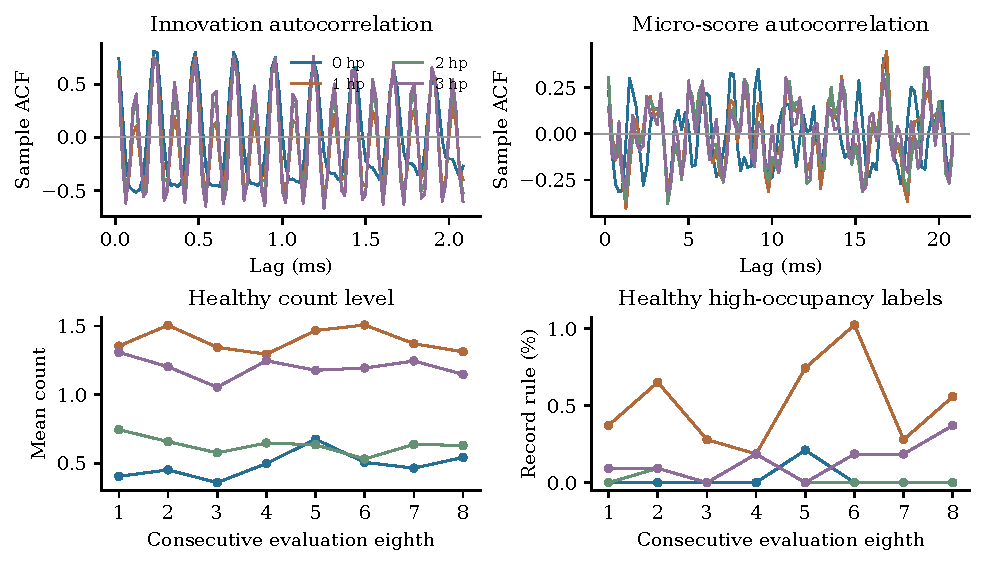
\includegraphics[width=\linewidth]{figures/cwru_reference_diagnostics.pdf}
\caption{Reference dependence and temporal variation. The upper panels use the chronological reference period. The lower panels divide each healthy evaluation sequence into eight consecutive groups of blocks. Adjacent groups may share raw observations at their boundaries because monitoring blocks overlap.}
\end{figure}

Short-lag correlation remains after fitting. Sample autocorrelations neither establish absolute regularity nor bound its coefficients. No numerical coupling allowance is attached to the nominal rank levels; larger gaps alone do not justify such an allowance.

Healthy fractions come from later parts of the four fitting recordings, not independent machines. The reproducibility files provide exact counts and denominators. We give no binomial confidence intervals, significance tests treating blocks as independent, or certified false-alarm rate. The unannotated episode durations also preclude evaluating duration coverage.

\clearpage
\subsection{Aggregation comparisons and count distributions}

For a block of scores \(Z_1,\ldots,Z_m\), the continuous comparators are
\[
 \frac{|\sum_jZ_j|}{\sqrt m},\quad
 \sum_j Z_j^2,\quad
 \sum_j\min(Z_j^2,c_0^2),\;
 \max_{\substack{1\le u\le v\le m\\v-u+1\ge3}}
 \frac{|\sum_{j=u}^vZ_j|}{\sqrt{v-u+1}},\;
 \max_{1\le j\le m-2}\min(|Z_j|,|Z_{j+1}|,|Z_{j+2}|).
\]
Each receives its own healthy \(190\)th and \(198\)th order-statistic cutoffs. Strict upper exceedance gives label 2. For an additional common-nominal comparison, we order pairs \((T,U)\) lexicographically with independent \(U\sim\mathrm{Unif}(0,1)\), and reject above the \(198\)th reference pair. This removes the count rule's two-count middle-class requirement and record floor. It targets the same nominal rank level, not equality of achieved dependent-data error rates.

\begin{table}[H]
\centering\small
\begin{tabular}{lrr}
\toprule
Statistic & Healthy (\%) & Primary faults (\%) \\
\midrule
Count & 1.156 & 96.512 \\
Block sum & 1.689 & 36.798 \\
Energy & 1.512 & 98.492 \\
Capped energy & 1.477 & 97.040 \\
Interval scan & 1.381 & 68.753 \\
Run statistic & 1.430 & 91.999 \\
\bottomrule
\end{tabular}
\caption{Common nominal \(.01\) randomized-rank comparison. The tie-breaking seed is 20261110, with separate streams by load, recording, and calibration/evaluation role. A direct and a record count cannot be distinct tests after imposing the same final count rule.}
\end{table}

\begin{figure}[H]
\centering
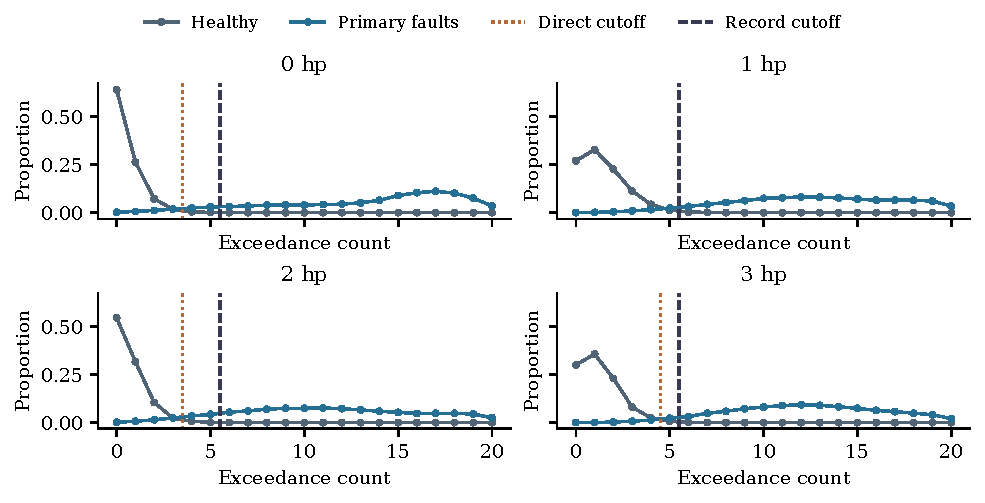
\includegraphics[width=.94\linewidth]{figures/cwru_count_distributions.pdf}
\caption{Empirical exceedance-count distributions. Fault curves average the nine primary faulty recordings at each load equally. Vertical lines separate counts below and above each upper threshold; at \(1\) hp the cutoffs coincide.}
\end{figure}

The distributions make the role of the floor explicit: it removes a band of moderate counts from the upper label. An externally chosen numerical floor with the same value would give exactly the same classifications. The record benchmark makes that preference reproducible; these data do not establish a unique performance advantage of its record-theoretic origin.


\bibliographystyle{plainnat}
\bibliography{references}
\end{document}
